We will now discuss two kinds of Jupyter Notebooks that use the MMT kernel and background theories from MathHub.info.
The first is an originary OpenDreamKit VRE application focused on computational mathematics as envisioned in the propsal, the second appeared in the course of the collaboration between WP2 (Micromagnetic VRE for modeling and simulation) and WP6. 

\subsection{MitM-Based Formalized Mathematics in MathHub Notebooks}

The MitM approach in  OpenDreamKit uses the MMT language for formalizing mathematical background knowledge and the MMT system for integrating computation tools.
Therefore, Jupyter-MMT notebooks can serve as a unified user interface for MitM systems.

For example, consider the theory at \url{https://gl.mathhub.info/ODK/lmfdb/blob/master/source/schemas/tutorial_example.mmt}, which serves as our standard example for the interaction between MMT and LMFD (a big database of mathematical objects that was integrated with MMT in previous deliverables of OpenDreamKit).
We can now rewrite it as a notebook.\ednote{@Kai: prepare the notebook, add a link and a screenshot here}

\begin{figure}[ht]\centering
  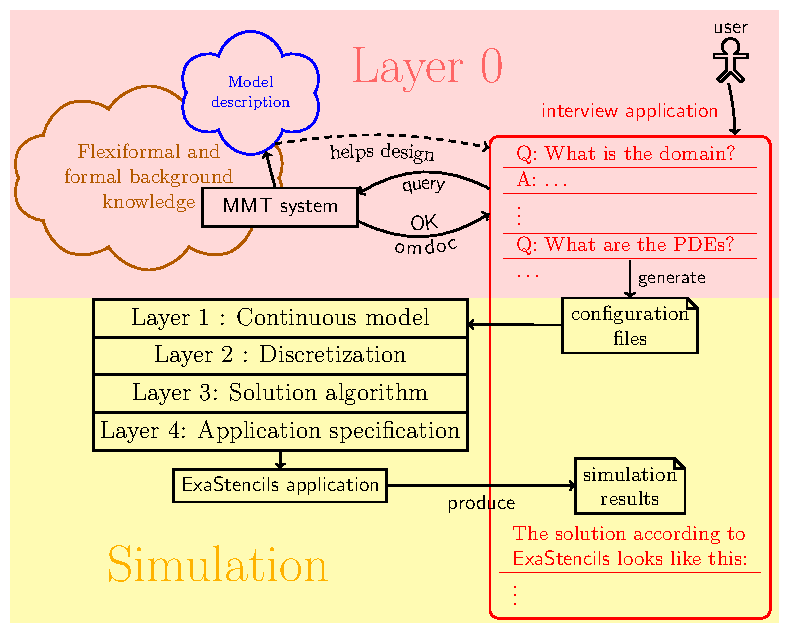
\includegraphics[width=0.6\textwidth]{proto}
  \caption{MoSIS Information Architecture}\label{fig:prototype}
\end{figure}

\subsection{Domain specific applications: MoSIS}

Our second case study addresses a \emph{knowledge gap} that is commonly encountered in computational science and engineering:

 To set up a simulation, we need to combine domain knowledge (usually in terms of physical principles), model knowledge (e.g. about suitable partial differential equations) with simulation (i.e. numerics/computing) knowledge.
In pre-VRE practice, this is resolved by intense collaboration between experts, which incurs non-trivial translation and communication overheads.
In OpenDreamKit propose an alternate solution, based on mathematical knowledge management (MKM) techniques, specifically a Jupyter notebook that has access to an OMDoc/MMT theory graph on MathHub.info: 

Given a theory graph representation of the domain, model, and background mathematics, we
can derive a targeted knowledge acquisition dialogue that supports the formalization of
domain knowledge, combines it with simulation knowledge and -- in the end -- drives a
simulation run all integrated into a Juypter Notebook.
Figure~\ref{fig:prototype} shows the general architecture:
The left side shows the simulation engine \textsf{ExaStencils} and the MMT system that acts as the theory graph interface.
The right hand side shows the interview – a Jupyter notebook – as the active document and how it interacts with the MMT kernel.
The user only sees the notebook; answers the knowledge acquisition questions presented by MoSIS, until MoSIS can generate a ExaStencils configuration file to be shipped to ExaStencils, which transforms it into efficient code through the ExaSlang layers, computes the results and visualizations, that MoSIS in turn incorporates into the notebook. 

\begin{figure}[ht]
  \fbox{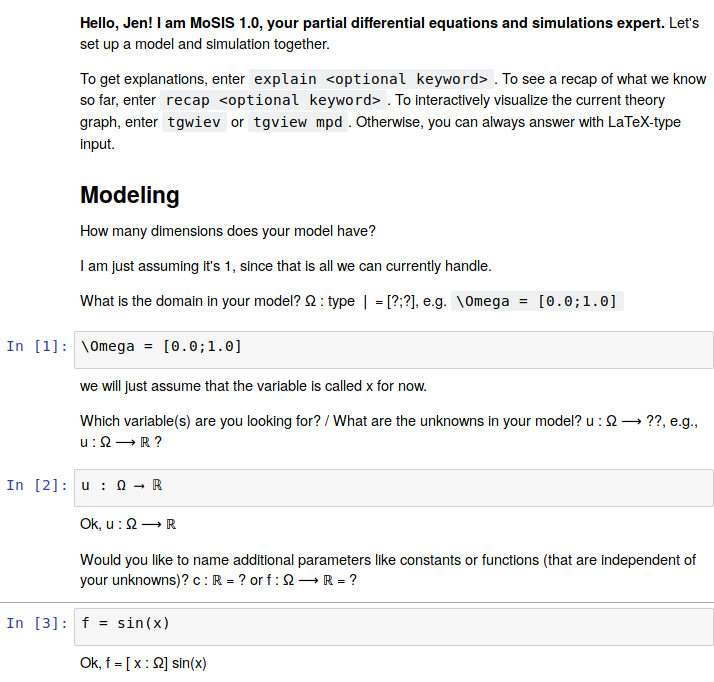
\includegraphics[width=0.8\textwidth]{Screenshot_interview}}
  \caption{Beginning of a Dialogue in MoSIS}\label{fig:int_begin}
\end{figure}

Figure~\ref{fig:int_begin} shows a screenshot of the notebook.
Finally, Figure~\ref{fig:pde-theory} shows the underlying theory graph of background knowlede about mathematical models and partial differential equations. \cite{PolKohKoe:kacse18} gives details about this case study from the MKM perspective; the Jupyter/MMT/Mathhub integration was the base of the interview application which hides the mathematical details from the user.  

\begin{figure}[h!p]\centering
  \begin{turn}{-90}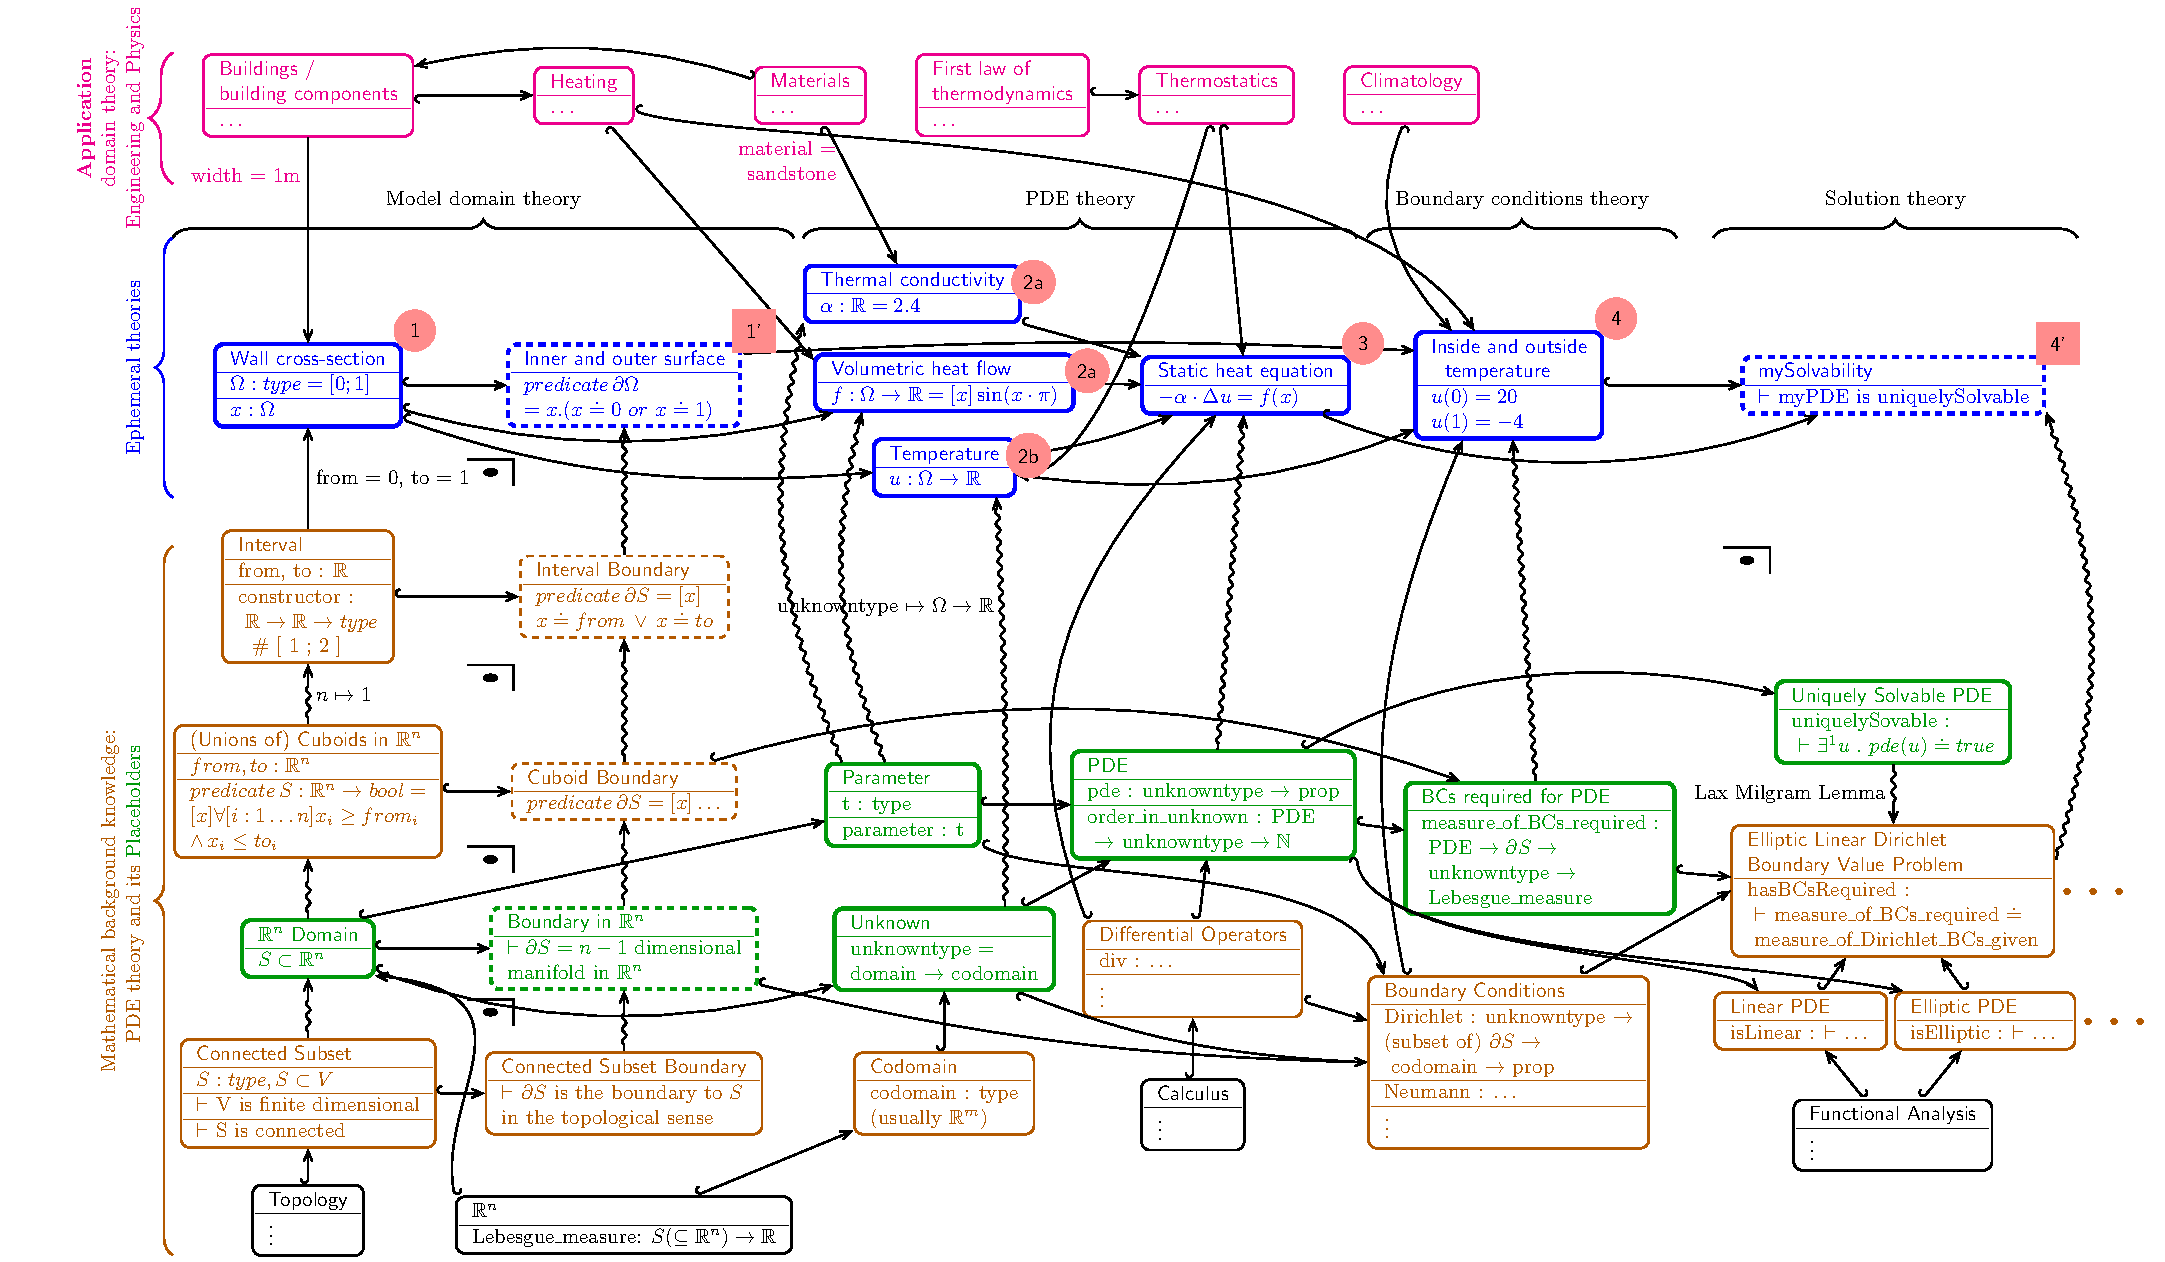
\includegraphics[width=0.95\textheight]{pde-theory}\end{turn}
  \caption{Theory Graph for the MoSIS Case Study}\label{fig:pde-theory}
\end{figure}

%%% Local Variables:
%%% mode: latex
%%% mode: visual-line
%%% fill-column: 5000
%%% TeX-master: "report"
%%% End:

%  LocalWords:  MitM-Based Formalized formalizing Jupyter-MMT ednote summarize
